\documentclass[11pt,a4paper,oldfontcommands]{memoir}

\usepackage[T1]{fontenc}
\usepackage[utf8]{inputenc}
\usepackage{lmodern}
\usepackage{microtype}
\usepackage[dvips]{graphicx}
\usepackage{xcolor}
\usepackage{times}
\usepackage{csquotes}
\usepackage{mathtools}
\usepackage[
breaklinks=true,colorlinks=true,
%linkcolor=blue,urlcolor=blue,citecolor=blue,% PDF VIEW
linkcolor=black,urlcolor=black,citecolor=black,% PRINT
bookmarks=true,bookmarksopenlevel=2]{hyperref}

\usepackage{geometry}
% PDF VIEW
% \geometry{total={210mm,297mm},
% left=25mm,right=25mm,%
% bindingoffset=0mm, top=25mm,bottom=25mm}
% PRINT
\geometry{total={210mm,297mm},
left=20mm,right=35mm,
bindingoffset=0mm, top=25mm,bottom=25mm}

\usepackage[textsize=tiny,textwidth=3cm]{todonotes}
\setlength{\marginparwidth}{3cm}

\linespread{1.5}

%%% CHAPTER'S STYLE
%\chapterstyle{bianchi}
%\chapterstyle{ger}
\chapterstyle{madsen}
%\chapterstyle{ell}
%%% STYLE OF SECTIONS, SUBSECTIONS, AND SUBSUBSECTIONS
\setsecheadstyle{\Large\bfseries\sffamily\raggedright}
\setsubsecheadstyle{\large\bfseries\sffamily\raggedright}
\setsubsubsecheadstyle{\bfseries\sffamily\raggedright}


%%% STYLE OF PAGES NUMBERING
\pagestyle{companion}\nouppercaseheads 
%\pagestyle{headings}
%\pagestyle{Ruled}
%\pagestyle{plain}
\makepagestyle{plain}
\makeevenfoot{plain}{\thepage}{}{}
\makeoddfoot{plain}{}{}{\thepage}
\makeevenhead{plain}{}{}{}
\makeoddhead{plain}{}{}{}


\maxsecnumdepth{subsection} % chapters, sections, and subsections are numbered
\maxtocdepth{subsection} % chapters, sections, and subsections are in the Table of Contents
\usepackage[french]{babel}
\begin{document}
\title{Développements instrumentaux et simulations Monte Carlo pour la détection des rayons gamma prompts pour le contrôle de l’hadronthérapie}
\author{Simon Martin}
\date{Juin 2020}



\maketitle
\newpage
\tableofcontents
\openany
\chapter{Introduction}
<<<<<<< HEAD
Les cancers sont aujourd'hui une des principales cause de mortalité en France et leur traitement est un des sujets de recherche majeur dans le panorama scientifique actuel. Parmi ces traitements les techniques utilisant des rayonnements ionisants (radiothérapies) sont utilisé dans près de 50\% des cas. L'hadronthérapie fait partie de ces techniques
: elle est utilisée dans le cas des tumeurs inopérables et/ou radiorésistantes. En utilisant des ions, cette technique permet d'atteindre une grande précision sur la dose déposée. Cependant cette précision est à double tranchant : en cas par exemple de mauvais positionnement du patient ou de changements morphologiques, le parcours des ions peut être sensiblement différent de celui qui a été planifié et conduire à un sous-dosage du volume tumoral et à un surdosage des tissus saints environnants. C'est pour résoudre ce problème que des solutions de contrôle en ligne du parcours des ions sont étudiées. Une de ces solutions serait de détecté les rayons gamma prompts émis lors des réactions nucléaires subies par une fraction des ions incidents (Prompt Gamma (PG) en anglais). C'est dans cette optique que des détecteurs spécifiques à cette utilisation sont en cours de développement. Des simulations capables de reproduire au mieux l'émission de PG de façon optimale sont développées en parallèle afin de concevoir et caractériser ces détecteurs. Nous introduirons tout d'abord dans ce rapport l'hadronthérapie pour ensuite nous concentrer sur la caractérisation de détecteur BGO servant dans un prototype de caméra PG et enfin nous présenterons le travail d'amélioration du module de simulation \enquote{vpgTLE} utilisé pour simuler l'émission et la détection des rayons PG. 
\openany
\section{Hadronthérapie}
L'hadronthérapie est une technique de traitement utilisant des faisceaux de protons et d'ions légers (comme les ions hélium, carbone et oxygène) et leurs propriétés physiques pour traiter les cancers avec une grande précision. Le préfixe \enquote{Hadron} dans hadronthérapie vient du fait que les particules utilisées pour irradier le patient sont des particules soumises à l'interaction forte. Actuellement les particules utilisées en traitement ainsi qu'en recherche sont des ions en très grande majorité, les neutrons étant peu utilisés et les pions ayant été mis à l'écart à la fin des années 80. Depuis 1946 et l'article pionnier de Robert Wilson dans Radiology\cite{wilson} sur l'intérêt thérapeutique des protons, le nombre de centres de protonthérapie a connu une croissance exponentielle(il existe actuellement une cinquantaine de centre de protonthérapie et une dizaine de centre utilisant des ions carbone). Bien que cette technique soit au stade de l'industrialisation aujourd'hui, des améliorations sont possibles autant sur le plan physique et biologique que technique. 
\subsection{Intérêts}
L'intérêt principal des ions réside dans la forme de la distribution de  dose qu'ils déposent dans le patient. En effet ils cèdent une grande partie de leur énergie dans les derniers millimètres de leur parcours formant ainsi ce que l'on appelle le pic de Bragg, contrairement à un faisceau de photons qui lui va céder son énergie de manière moins localisé. C'est ce pic de Bragg qui va permettre aux ions de déposer la dose plus localement et d'être plus précis que les photons, épargnant ainsi les tissus sains proches de la tumeur comme le montre la figure \ref{CvsG}. La profondeur de ce pic peut être ajustée via l'énergie des ions envoyés alors que la position du faisceau est contrôlé par un système de champ magnétique (dans le cas d'une délivrance active du faisceau). La précision de cette technique lui permet d'être utilisée dans des cas où des organes à risque se trouvent proches de la tumeur, notamment pour des cancers oculaires ou spinaux et plus généralement les cancers de la zone ORL. La protonthérapie est également prescrite dans les cas de cancer pédiatrique. En effet les tissus en développement chez l'enfant étant plus radiosensibles que ceux de l'adulte, il est absolument nécessaire de minimiser autant que possible la dose déposée dans ces tissus. \\
\begin{figure}
    \centering
    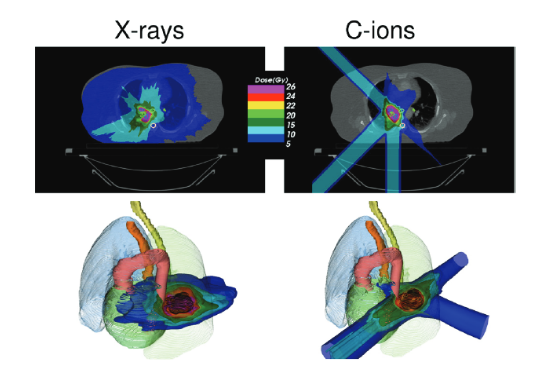
\includegraphics[scale = 0.7]{intro/xrvshDuranteetal2016.png}
    \caption{Comparaison entre un plan de traitement de rayons X et d'ions carbone \cite{Durante_2016}}
=======
Les cancers sont aujourd'hui une des principales cause de mortalité en France et leur traitement est un des sujets de recherche majeur dans le panorama scientifique actuel. Parmi ces traitements, les techniques utilisant des rayonnements ionisants (radiothérapie) sont utilisé dans près de 50\% des cas. L'hadronthérapie fait partie de ces techniques : elle est utilisée dans le cas des tumeurs inopérables et/ou radiorésistantes. En utilisant des ions, cette technique permet d'atteindre une grande précision sur la dose déposée. Cependant cette précision est à double tranchant : en cas par exemple de mauvais positionnement du patient ou de changements morphologiques, le parcours des ions peut être sensiblement différent de celui qui a été planifié et conduire à un sous-dosage du volume tumoral et à un sur-dodage des tissus sains environnants. C'est pour résoudre ce problème que des solutions de contrôle en ligne du parcours des ions sont étudiées. Une de ces solutions serait de détecter les rayons gamma prompts émis lors des réactions nucléaires subies par une fraction des ions incidents (Prompt Gamma (PG) en anglais). C'est dans cette optique que des détecteurs spécifiques à cette utilisation sont en cours de développement. Des simulations capables de reproduire au mieux l'émission des PG de façon optimale sont développées en parallèle afin de concevoir et caractériser ces détecteurs. Nous introduirons tout d'abord dans ce rapport l'hadronthérapie pour ensuite nous concentrer sur la caractérisation de détecteur BGO servant dans un prototype de caméra PG et enfin nous présenterons le travail d'amélioration du module de simulation \enquote{vpgTLE} utilisé pour simuler l'émission et la détection des rayons PG.

\openany
\section{Hadronthérapie}
L'hadronthérapie est une technique de traitement utilisant des faisceaux de protons et d'ions légers (comme les ions hélium, carbone et oxygène) et leurs propriétés physiques pour traiter les cancers avec une grande précision. Le préfixe \enquote{hadron} dans hadronthérapie vient du fait que les particules utilisées pour irradier le patient sont des particules soumises à l'interaction forte. Actuellement les particules utilisées en traitement ainsi qu'en recherche sont des ions en très grande majorité, les neutrons étant peu utilisés et les pions ayant été mis à l'écart à la fin des années 80. Depuis 1946 et l'article pionnier de Robert Wilson dans Radiology\cite{wilson} sur l'intérêt thérapeutique des protons, le nombre de centres de protonthérapie a connu une croissance exponentielle (il existe actuellement une cinquantaine de centre de protonthérapie et une dizaine de centre utilisant des ions carbone). Bien que cette technique soit au stade de l'industrialisation aujourd'hui, des améliorations sont possibles autant sur le plan physique et biologique que technique. 
\subsection{Intérêts}
L'intérêt principal des ions réside dans la forme de la distribution de dose qu'ils déposent dans le patient. En effet, ils cèdent une grande partie de leur énergie dans les derniers millimètres de leur parcours formant ainsi ce que l'on appelle le pic de Bragg, contrairement à un faisceau de photons qui lui va céder son énergie de manière moins localisé. C'est ce pic de Bragg qui va permettre aux ions de déposer la dose plus localement et d'être plus précis que les photons, épargnant ainsi les tissus sains proches de la tumeur comme le montre la figure \ref{CvsG}. La profondeur de ce pic peut être ajustée via l'énergie des ions envoyés alors que la position du faisceau est contrôlé par un système de champ magnétique (dans le cas d'une délivrance active du faisceau). La précision de cette technique lui permet d'être utilisée dans des cas où des organes à risque se trouvent proches de la tumeur, notamment pour des cancers oculaires ou spinaux et plus généralement les cancers de la zone ORL. La protonthérapie est également prescrite dans les cas de cancer pédiatrique. En effet, les tissus en développement chez l'enfant étant plus radiosensibles que ceux de l'adulte, il est absolument nécessaire de minimiser autant que possible la dosée déposée dans ces tissus. \\

\todo{Citer la référence : cite{ref} dans la figure \ref{CvsG}} 
\begin{figure}
    \centering
    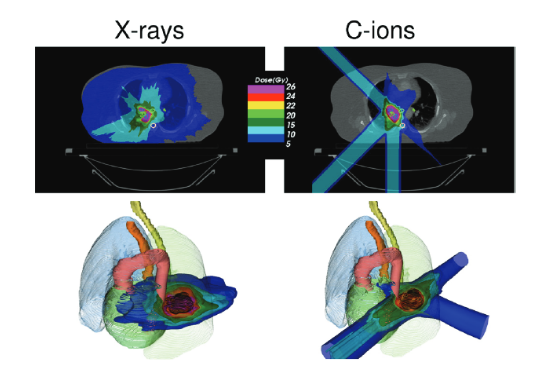
\includegraphics[scale = 0.7]{intro/xrvshDuranteetal2016.png}
    \caption{Comparaison entre un plan de traitement de rayons X et d'ions carbone (Durante et al. 2016)}
>>>>>>> b7684bc6d0fea1fa9dda550dcd57d627ca07c078
    \label{CvsG}
\end{figure}

On définit l'efficacité biologique relative (EBR) comme le ratio entre les doses nécessaires pour obtenir le même effet biologique avec un faisceau d'ions et un faisceau de photons
$$EBR = \frac{D_{photon}}{D_{ion}}\bigg|_{\mathrm{effet}}$$
C'est une quantité complexe qui dépend de beaucoup de facteurs et notamment du poids des particules. Plus les particules sont lourdes plus la densité d'ionisations dans la cible est élevée. Or les dommages causés par les ions sont directement liés à la densité d'ionisations est directement. De plus la position des interactions des photons dans la matière sont aléatoires alors que, dans le cas des ions, ces interactions se font tout au long de leur parcours. Ils créent donc des zones où la densité d'ionisations est élevée, particulièrement dans la région du pic de Bragg. Ce phénomène est illustré dans la figure \ref{LET} où l'on voit que la concentrations de cassures double brin est importante sur le parcours des ions alors qu'elle est plus disparate pour les photons. On considère globalement que l'EBR dans la zone tumorale esy d'environ 1.1 pour les protons et compris entre 2 et 5 pour les ions carbone cite{Choi}. 

<<<<<<< HEAD
On définit l'efficacité biologique relative (EBR) comme le ratio entre les doses nécessaires pour obtenir le même effet biologique avec un faisceau d'ions et un faisceau de photons.
$$EBR = \frac{D_{photon}}{D_{ion}}\bigg|_{\text{effet}}$$
C'est une quantité complexe qui dépend de beaucoup de facteurs et notamment du poids des paticules. Plus les particules sont lourdes plus la densité d'ionisations dans la cible est élevé. Or les dommages causés par les ions sont directement liés à la densité d'ionisations. De plus la position des interactions des photons dans la matière sont aléatoires, dans le cas des ions ces interactions se font tout au long de leur parcours. Ils créent donc des zones où la densité d'ionisation est élevée, particuliérement dans la région du pic de Bragg. Ce phénomène est illustré dans la figure \ref{LET} où l'on voit que la concentrations de cassures double brin est importante sur le parcours des ions alors qu'elle est plus disparate pour les photons. On considère globalement que l'EBR dans la zone tumorale est d'environ 1.1 pour les protons et compris entre 2 et 5 pour les ions carbone\cite{Choi}. 
=======
\todo{Citer la référence : cite{ref} dans la figure \ref{LET}} 
>>>>>>> b7684bc6d0fea1fa9dda550dcd57d627ca07c078
\begin{figure}
    \centering
    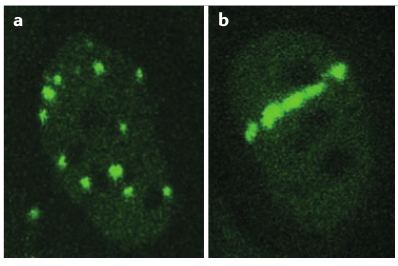
\includegraphics[scale = 0.7]{intro/LETDSS.png}
    \caption{Concentration des cassures doubles brins dans une cellule de culture prélever d'un osteosacrome chez un patient pour (a) une exposition à des rayons X et (b) à des ions carbone. Les cassures double brins sont visualisé grâce à de l'immunofluorescence marquant les histones $ \gamma$ H2AX \cite{Durante2017}}
    \label{LET}
\end{figure}

\subsection{Défis}
Malgré l'augmentation du nombre de centres et une industrialisation progressive de la technique, l'hadronthérapie reste une technique coûteuse et sa rentabilité est difficile à évaluer \cite{LIEVENS2013134}. Un centre d'hadronthérapie peut coûter entre 3 fois (pour la protonthérapie), et 7 fois (pour la thérapie par ions carbone), plus cher qu'un centre de traitement par rayons X dernière génération \cite{Nupecc}. Des avancées pour rendre les accélérateurs plus compacts et moins chers sont donc encore nécessaires.


<<<<<<< HEAD
Les propriétés balistiques des ions ne sont pas encore exploitées de façon optimale, la technique étant très sensible aux changement morphologiques, aux erreurs de positionement ainsi qu'aux incertitudes de conversion des unitées hounsfield (obtenues à partir d'images scanner) en cartes de pouvoir d'arrêt des ions (nécessaires pour effectuer la plannification de traitement)\cite{Paganetti2012}. Une marge de sécurité pouvant atteindre 10~mm est donc appliqué au volume cible planifié. Cette marge pourrait être réduite en utilisant des moyens de contrôle en ligne tels que l'imagerie TEP \cite{Parodi20157153} ou Prompt Gamma \cite{PGMonitoringC12}. Nous nous intéresserons plus particulièrement aux techniques \enquote{Prompt Gamma} dans la suite de ce rapport. \\
Des simulations visant à être plus rapide que les simulations MC classiques tout en restant aussi précises sont en cours de développement \cite{Huisman_2016}\cite{Embriaco_2018}\cite{Sterpin_2015}. Ce genre de simulations est nécessaire pour comparer les distributions PG mesurées aux distributions attendues et déterminer ainsi si le traitement s'est déroulé comme prévu ou pas.

\section{Création et délivrance d'un faisceau d'ion}
Les premiers accélérateurs utilisé en hadronthérapie étaient destinés en première intention à la physique nucléaire et à la physique des particules. Ils n'étaient donc pas vraiment adaptés aux irradiations médicales. Pour pouvoir traiter des lésions profondes, l'énergie du faisceau d'ions doit être modulable de façon à pouvoir atteindre une profondeur allant jusqu'à 25 cm. Ce faisceau doit également être capable d'être déplacé précisément dans le plan perpendiculaire à sa direction de propagation pour pouvoir impacter tout le volume à traiter. Pour satisfaire ces conditions deux méthodes d'accélération sont utilisées actuellement, le cyclotron, principalement utilisé en protonthérapie, et le synchrotron, utilisé pour les ions.

Un cyclotron est composé de deux électrodes vides. Une tension variant de façon alternative est appliquée entre elles et permet d'accélérer les particules chargées. Un champ magnétique perpendiculaire au plan du cyclotron permet d'obtenir une trajectoire circulaire. Le faisceau ainsi créé possède une intensité fixe avec une énergie fixe. Pour pouvoir faire varier cette énergie, et régler ainsi la profondeur du pic de Bragg, on utilise un système passif sur la ligne du faisceau. Ce système est composé d'un diffuseur qui va élargir le faisceau relativement étroit en un faisceau homogène et large et d'un dégradeur qui va venir étaler le pic de Bragg. Il va pouvoir ainsi traiter sur toute une gamme de profondeur. Un compensateur situé au niveau de la peau du patient qui va venir limiter le faisceau à la forme du volume traité.

Les synchrotrons, eux, utilisent une trajectoire dont le rayon de courbure est maintenu fixe grâce à un champs magnétique qui varie de façon à garder la particule dans leur enceinte jusqu'à ce qu'elle atteigne l'énergie voulue. Contrairement aux cyclotrons, les synchrotrons ont la possibilité de faire varier rapidement l'énergie du faisceau délivré sans système externe mais présente une intensité plus faible. Les synchrotrons sont également beaucoup moins compacts ; ils font une taille de 10~m pour les protons et 30~m pour les ions carbone. Un système actif de délivrance du faisceau sera privilégié pour répartir la dose: ce système est composé de deux aimants permettant d'orienter la trajectoire du faisceau dans le plan perpendiculaire à la direction de propagation du faisceau. La profondeur est quant à elle réglée via l'énergie du faisceau. Ce système permet une meilleure conformité du faisceau et n'utilise pas de matériel externe dépendant du patient, ce qui permet de réduire la dose induite par les neutrons secondaires générés dans les éléments interceptant le faisceau (diffuseur et dégradeur). L'inconvénient est que ce type de système de délivrance du faisceau est plus sensible aux mouvements d'organe. 
=======
Les propriétés balistiques des ions ne sont pas encore exploitées de façon optimale, la technique étant très sensible aux changement morphologiques, aux erreurs de positionnement ainsi qu'aux incertitudes de conversion des unitées hounsfield (obtenues à partir d'images scanner) en cartes de pouvoir d'arrêt des ions (nécessaires pour effectuer la planification de traitement) \cite{Paganetti2012}. Une marge de sécurité pouvant atteindre 10~mm est donc appliqué au volume cible planifié. Cette marge pourrait être réduite en utilisant des moyens de contrôle en ligne tels que l'imagerie TEP (Tomographie à émission de positons) \cite{Parodi2018} ou \enquote{Prompt Gamma} \cite{Krimmer2017a}. Nous nous intéresserons plus particulièrement aux techniques \enquote{Prompt Gamma} dans la suite de ce rapport. \\
Des simulations visant à être plus rapide que les simulations MC classiques tout en restant aussi précises sont en cours de développement \cite{Huisman_2016}\cite{Embriaco_2018}\cite{Sterpin_2015}. Ce genre de simulations est nécessaire pour comparer les distributions PG mesurées aux distributions attendues et déterminer ainsi si le traitement s'est déroulé comme prévu ou pas.

\section{Création et délivrance d'un faisceau d'ion}
Les premiers accélérateurs utilisé en hadronthérapie étaient destinés en première intention à la physique nucléaire et à la physique des particules. Ils n'étaient donc pas vraiment adapatés aux irradiations médicales. Pour pouvoir traiter des lésions profondes, l'énergie du faisceau d'ions doit être modulable de façon à pouvoir atteindre une profondeur allant jusqu'à 25 cm. Ce faisceau doit également être capable d'être déplacé précisément dans le plan perpendiculaire à sa direction de propagation pour pouvoir impacter tout le volume à traiter. Pour satisfaire ces conditions deux méthodes d'accélération sont utilisées actuellement, le cyclotron, principalement utilisé en protonthérapie, et le synchrotron, utilisé pour les ions.

Un cyclotron est composé de deux électrodes vides. Une tension variant de façon alternative est appliquée entre elles et permet d'accélérer les particules chargées. Un champ magnétique perpendiculaire au plan du cyclotron permet d'obtenir une trajectoire circulaire. Le faisceau ainsi créé possède une intensité fixe avec une énergie fixe. Pour pouvoir faire varier cette énergie, et régler ainsi la profondeur du pic de Bragg, on utilise un système passif \todo{Non : tu confonds système passif et réglage de l'énergie avec un dégradeur} sur la ligne du faisceau. Ce système est composé d'un diffuseur qui va élargir le faisceau relativement étroit en un faisceau homogène et large et d'un dégradeur qui va venir étaler le pic de Bragg. Il va pouvoir ainsi traiter sur toute une gamme de profondeur. Un compensateur situé au niveau de la peau du patient qui va venir limiter le faisceau à la forme du volume traité \todo{Non}. 

Les synchrotrons, eux, utilisent une trajectoire dont le rayon de courbure est maintenu fixe grâce à un champs magnétique qui varie de façon à garder la particule dans leur enceinte jusqu'à ce qu'elle atteigne l'énergie voulue. Contrairement aux cyclotrons, les synchrotrons ont la possibilité de faire varier rapidement l'énergie du faisceau délivré sans système externe mais présente une intensité plus faible. Les synchrotrons sont également beaucoup moins compacts ; ils font une taille de 10~m pour les protons et 30~m pour les ions carbone. Un système actif de délivrance du faisceau sera privilégié pour répartir la dose: ce système est composé de deux aimants permettant d'orienter la trajectoire du faisceau dans le plan perpendiculaire à la direction de propagation du faisceau\todo{ça existe aussi en proton\dots}. La profondeur est quant à elle réglée via l'énergie du faisceau. Ce système permet une meilleure conformité du faisceau et n'utilise pas de matériel externe dépendant du patient, ce qui permet de réduire la dose induite par les neutrons secondaires générés dans les éléments interceptant le faisceau (diffuseur et dégradeur). L'inconvénient est que ce type de système de délivrance du faisceau est plus sensible aux mouvements d'organe. 
>>>>>>> b7684bc6d0fea1fa9dda550dcd57d627ca07c078

\begin{figure}[h!]
    \centering
    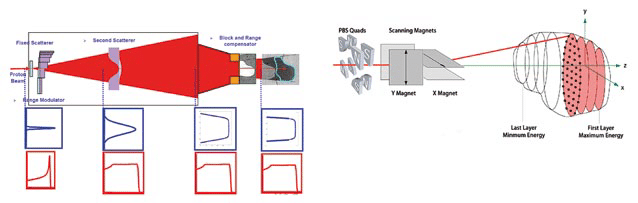
\includegraphics [scale = 0.7]{intro/Passive-left-and-active-right-beam-delivery-system-courtesy-of-IBA.png}
    \caption{Comparaison entre un système de délivrance du faisceau passif (gauche) et actif (droite) (Rapport Nupecc 2014)}
    \label{fig:my_label}
\end{figure}
\openany
\section{Interaction ion-matière}
\subsection{Physique des interactions}

<<<<<<< HEAD
Il est possible de séparer les interactions entre les ions et la matière en 2 catégories, la première correspondant aux interactions entre les ions et les atomes et la seconde aux interactions entre les ions et les noyaux de ces même atomes. L'interaction entre un ions et l'atome est de type électromagnétique (EM) inélastique. La deuxième catégorie regroupe deux interaction, une première EM élastique et une deuxième nucléaire. D'autres interactions sont possibles mais sont négligeables dans le cadre de l'hadronthérapie.\\
=======
%\todo{Cela n'a pas de sens de parler d'interaction inélastique avec les électrons puisque les électrons sont des particules élémentaires qui ne peuvent avoir d'énergie interne d'excitation. Il faut parler de collisions inélastiques avec les atomiques cibles ou d'interaction avec les électrons.}\todo{Je pense qu'il est plus juste et plus simple de distinguer les interactions avec les électrons (en fait avec les atomes ou molécules) et les interactions avec les noyaux atomiques. Pour éventuellement détailler ensuite les différents types de ces 2 grands types d'interactions.}
Il est possible de séparer les interactions entre les ions et la matière en 2 catégories, la première correspondant aux interactions entre les ions et le nuage électronique des atomes et la seconde aux interactions entre les ions et les noyaux de ces même atomes. L'interaction entre un ions et le nuage électronique est de type électromagnétique (EM) inélastique. La deuxième catégorie regroupe deux interaction, une première EM élastique et une deuxième nucléaire. D'autres interactions sont possibles mais sont négligeables dans le cadre de l'hadronthérapie.\todo{à revoir}\\
>>>>>>> b7684bc6d0fea1fa9dda550dcd57d627ca07c078
\begin{figure}[h!]
    \centering
    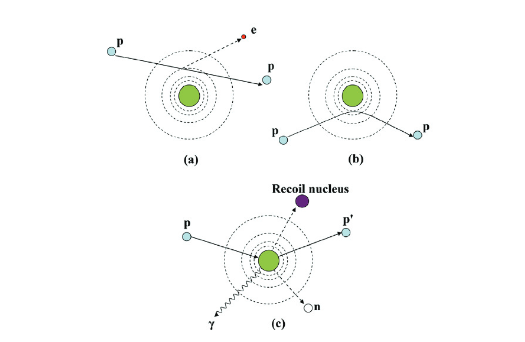
\includegraphics{intro/Newhauser2015.PNG}
    \caption{Schéma des différentes interactions d'un protons dans la matière: EM inélastique (a), EM élastique (b) et nucléaire (c) (Newhauser et. al 2015)}
    \label{fig:my_label}
\end{figure}

<<<<<<< HEAD
Les interactions EM inélastiques avec le nuage électronique sont la principale source de perte d'énergie des ions.  Cette perte d'énergie peut être estimée à l'aide de la formules de Bethe et Bloch. La dépendance du pouvoir d'arrêt en $1/\beta^2$ (avec $\beta = \frac{v}{c}$, $v$ et $c$ les vitesses de l'ion et de la lumière respectivement) implique que plus la particule est rapide plus le pouvoir d'arrêt est faible. Le pouvoir d'arrêt maximal est atteint à la profondeur du pic de Bragg pour une vitesse égale à $v_p = z^{\frac{2}{3}}v_0$ (avec $v_0 = e^2/\hbar$ la vitesse de Planck, $e$ la charge électrique élémentaire, $\hbar$ la constante de Planck réduite et $z$ le numéro atomique de la particule) pour laquelle l'ion est suffisamment lent pour capturer des électrons et voir sa charge diminuer rapidement. 

Bien qu'ayant une part moins importante les interactions coulombienne avec les noyaux de la cible participent également à la distribution de la dose. Elles ont notamment un rôle important dans la diffusion latérale du faisceau.

En plus des interactions EM, les réactions nucléaires jouent un rôle important dans le dépôt de dose car elles produisent des rayonnements secondaires à l'origine d'une disperion partielle de la dose, notamment par les neutrons secondaires. Ces interactions peuvent être décrites en deux étapes : une première étape où l'ion entre en collision avec le noyau cible et une deuxième où les noyaux excités produit lors de la réaction se désexcitent en émettant des particules secondaires. En général, seule une partie des nucléons sont impliqués dans le processus de collision. Ces nucléons créent ainsi une zone appelée \enquote{boule de feu} tandis que les nucléons spectateurs forment des fragments \enquote{projectile ressemblant} et \enquote{cible ressemblant}. Ce sont tous ces fragments qui émettent des particules secondaires notamment des protons, des neutrons et des rayons gamma appelés \enquote{gammas prompts}.
=======
Les interactions EM inélastiques avec le nuage électronique sont la principale source de perte d'énergie des ions.  Cette perte d'énergie peut être estimée à l'aide de la formule de Bethe-Bloch. La dépendance du pouvoir d'arrêt en $1/\beta^2$ (avec $\beta = \frac{v}{c}$, $v$ et $c$ les vitesses de l'ion et de la lumière, respectivement) implique que plus la particule est rapide plus le pouvoir d'arrêt est faible. Le pouvoir d'arrêt maximal est atteint à la profondeur du pic de Bragg pour une vitesse égale à $v_p = z^{\frac{2}{3}}v_0$ (avec $v_0 = e^2/\hbar$ la vitesse de Planck, $e$ la charge électrique élémentaire, $\hbar$ la constante de Planck réduite et $z$ le numéro atomique de la particule) pour laquelle l'ion est suffisamment lent pour capturer des électrons et voir sa charge diminuer rapidement. 

Bien qu'ayant une part moins importante les interactions coulombienne avec les noyaux de la cible participent également à la distribution de la dose. Elles ont notamment un rôle important dans la diffusion latérale du faisceau.

En plus des interactions EM, les réactions nucléaires jouent un rôle important dans le dépôt de dose car elles produisent des rayonnements secondaires à l'origine d'une dispersion partielle de la dose, notamment par les neutrons secondaires. Ces interactions peuvent être décrites en deux étapes : une première étape où l'ion entre en collision avec le noyau cible et une deuxième où les noyaux excités produits lors de la réaction se désexcitent en émettant des particules secondaires. En général, seule une partie des nucléons sont impliqués dans le processus de collision. Ces nucléons créent ainsi une zone appelée \enquote{boule de feu} tandis que les nucléons spectateurs forment des fragments \enquote{projectile ressemblant} et \enquote{cible ressemblant}. Ce sont tous ces fragments qui émettent des particules secondaires, notamment des protons, des neutrons et des rayons gamma appelés \enquote{gammas prompts}. %Ces gammas proviennent de trois sources différentes; les prompt gammas issu de la désexcitation direct des noyaux, les gammas issus de l'annihilation de positrons émis par les noyaux et  les gammas issu de l'interaction entre les neutrons émis par les noyaux et la cible. Les deux première sortent de gamma sont utilisé pour le contrôle de l'hadronthérapie tandis que les gammas issu de neutrons participe au bruit de fond.


>>>>>>> b7684bc6d0fea1fa9dda550dcd57d627ca07c078
\openany
\section{Contrôle du parcours des ions lors de l'hadronthérapie}

\subsection{\'Etat de l'art}

Deux techniques majeures sont aujourd'hui étudiées : la première utilise les rayons gamma issus de l'annihilation de positons produits par des noyaux radioactif émmetteur $\beta^+$, qui peuvent eux mêmes être produit par une intéraction avec un ion, et l'autre basé sur la détection de gammas prompts. Nous nous intéressons plus particulièrement à cette dernière mais une description détaillé du contrôle TEP peut être trouvée dans Parodi (2015) \cite{Parodi20157153}. La détection de gammas prompts pour le contrôle de l'hadronthérapie est une technique prometteuse car d'une part le gammas sont émis très rapidement, moins d'une nanoseconde après l’interaction nucléaire entre un ion et sa cible, et d'autre part la corrélation du profil gamma prompts avec celui de la dose a été vérifié par \cite{PGMonitoringC12}pour les ions carbone et par \cite{Min2006} pour les protons. Plusieurs propositions ont été émise pour la détection de ces gammas et plusieurs prototypes existe dans le monde aujourd'hui. Ces prototypes peuvent être séparés en deux catégories, ceux produisant une image et ceux qui n'en produise pas. Dans la première catégorie une collimation est nécessaire pour obtenir une image après reconstruction, elle peut être de deux types, physique, en utilisant un collimateur matériel ou électronique à l'aide d'une caméra Compton. 

<<<<<<< HEAD
\subsubsection{Caméra Collimatée}
La caméra collimatée utilise une collimation physique discriminant les photons arrivant dans le détecteur sur leur endroit d'émission et obtenir ainsi une information spatiale sur le parcours des ions. Pour maximiser l’efficacité de détection tout en fournissant l'information sur la profondeur de l’émission des PG cette collimation ne se fait que sur une dimension. Deux types de collimateur sont étudiés par quelque groupe dans le monde : des collimateurs multi-fentes \cite{Pinto_2014,MinSimu} et un collimateur à une seule fente (\enquote{knife-edge slit} en anglais KES)\cite{Smeets_2012} fonctionnant sur le principe de la chambre noir.\\
Dans les deux cas les fentes sont composées d'un matériau lourd, comme un alliage de tungsten, afin de maximiser l'absorption de photon. 
La caméra KES \enquote{HiCam} dévellopé par IBA et un goupe du centre polytechnique de Milan et a été testé en conditions clinique avec des résultats prometteur \cite{Richter2016}.

\subsubsection{Caméra Compton}
Pour améliorer l’efficacité de détection des PG, plusieurs caméras Compton sont développés par plusieurs groupe dans le monde. Ce type de caméra permet de se passer d'un collimateur physique en ayant recourt au principe de collimation électronique basé sur la détection d'une interaction Compton et d'une absorption totale dans la caméra. Une image pourra être ensuite reconstruite à l'aide des cônes de réponses obtenu grâce a la cinématique Compton en utilisant les positions d’interactions et l'énergie déposée par celles-ci. Cette méthode de détection est bien adaptée à la détection de rayons gamma prompts car ceux ci sont émis avec des énergie de l'ordre de quelques MeV favorisant l'interaction Compton. Dans sa configuration la plus simple la caméra Compton se compose de deux éléments, un diffuseur et un absorbeur. Dans cette configuration l'absorption totale du photon dans l'absorbeur est nécessaire, on peut palier à ce problème en ajoutant un diffuseur au prix cependant d'une perte majeure d'efficacité de détection. Le désavantage majeur de cette technique est qu'a intensité clinique les coïncidences sont dominé par les coïncidences fortuites ce qui limite son utilisation a des intensités réduites. Des études sont en cours pour distinguer les vraies coïncidences des coïncidences fortuites grâce à l'intelligence artificielle \cite{Fontana_2020}. Dans leurs configurations actuelles les caméras Compton offrent un efficacité de détection comparable aux caméras collimatées qui ne détectent que sur une dimension, des optimisations de la géométrie sont en cours d'étude pour rendre le système compétitif. 
=======

\subsubsection{Caméra collimatée}

Les caméras collimatées développées pour le contrôle de l'hadronthérapie utilise en général une collimation 1D pour maximiser l'efficacité de détection tout en fournissant une information sur la distribution en profondeur de l'émission des PG. Deux types de collimateurs sont étudiés par quelques groupes dans le monde : des collimateurs multi-fentes \cite{Pinto_2014,MinSimu} et un collimateur à une seule fente (\enquote{knife-edge slit} en anglais, KES) \cite{Smeets_2012} fonctionnant sur le principe de la chambre noir. Dans les deux cas, le collimateur est composé d'un matériau lourd comme un alliage de tungstène afin de maximiser l'absorption totale des photons. \\
La caméra KES (\enquote{HiCam}) a été développé par la société IBA et un groupe du centre polytechnique de Milan et a été testée en conditions cliniques avec des résultats prometteurs \cite{Richter2016}. 

\subsubsection{Caméra Compton}

Pour améliorer l'efficacité de détection des PG, plusieurs caméras Compton sont développés par plusieurs groupes dans le monde. Ce type de caméra permet en effet de se passer d'un collimateur physique en ayant recours au principe de la collimation électronique basé sur la détection d'une diffusion Compton et d'une absorption totale du photon dans la caméra. A partir de la position et de l'énergie déposée lors de ces interactions, on peut déterminer l'angle d'incidence des photons incidents sur la caméra grâce à l'équation de la diffusion Compton. Cette angle d'incidence correspond à un cône dont l'axe est déterminé par la position des points d'interaction du photon dans la caméra. Cette méthode de détection est bien adaptée à la détection de rayons gamma prompts car ceux-ci sont étant émis avec des énergies relativement élevées de l'ordre de quelques MeV favorisant l'interaction Compton. Dans sa configuration la plus simple la caméra Compton se compose de deux éléments, un diffuseur et un absorbeur. Dans cette configuration, l'absorption totale du photon dans l'absorbeur est nécessaire, on peut palier à ce problème en ajoutant un diffuseur au prix cependant d'une perte majeure d'efficacité de détection. 

Manque des informations importantes : \todo{A rédiger} 
\begin{itemize}
  \item coïncidences dominées par les coïncidences fortuites à intensité clinique $\Rightarrow$ nécessité de fonctionner à intensité réduite sauf si l'on arrive à distinguer les coïncidences vraies des coïncidences fortuites grâce à de l'intelligence artificielle (Fontana IEEE TRMS 2019). 
  \item Efficacité de détection comparable à celle des caméras collimatées (qui \enquote{boostent} leur efficacité en ne faisant que de la collimation 1D $\Rightarrow$ nécessité d'augmenter l'efficacité de détection (travail en cours d'Ane).
\end{itemize}




\subsubsection{Systèmes de contrôle sans collimation (physique ou électronique)}

Certains groupes de recherche ont cherché à développer des systèmes plus légers que les caméras collimatées ou Compton et donc plus facilement intégrables à un environnement clinique. Ces systèmes ont pour objectif de contrôler le parcours des ions avec un ou plusieurs détecteurs placés autour du patient qui mesurent l'énergie des photons et/ou le temps de vol, c'est-à-dire le temps entre l'arrivée d'un ion incident et la détection d'un  PG (\enquote{Time of Flight} ou ToF en anglais). 

La technique PGT (\enquote{Prompt Gamma Timing}) initiée par \cite{Golnik_2014} utilise le lien qui existe entre la distribution de TOF des PG et le parcours des protons. En effet, plus le parcours des ions est important, plus la distribution de TOF des PG est large. Des différences de parcours allant jusqu'à 2~mm pour des fantômes hétérogènes ont put être détectées \cite{Hueso_Gonz_lez_2015}. Avec une mesure de TOF extrêmement précise (avec des résolutions temporelles de l'ordre de 100~ps RMS), il est même possible de reconstruire le point d'émission des PG uniquement à partir de cette information temporelle : c'est le projet TIARA.\todo{A développer}

La technique PGPI (\enquote{Prompt Gamma Peak Integral}) est basée sur le comptage des PG détectés par quelques détecteurs placés autour du patient. Les PG sont sélectionnés par mesure de TOF et le nombre de PG est obtenu en calculant l'intégral du \enquote{pic PG} dans la distribution de TOF mesurée (d'où le nom de la technique). Le nombre total de PG détectés par l'ensemble des détecteurs ainsi que les rapports des nombres de PG détectés dans les différents détecteur fournissent une information spatiale le parcours des ions.

Enfin, le principe technique PGS (\enquote{Prompt Gamma Spectroscopy}) est de mesurer le spectre des PG émis à la fin du parcours avec un détecteur collimaté \cite{Testa_2014}.  Le spectre d'énergie des PG varie en effet rapidement avec l'énergie des protons quand ceux-ci sont en fin de parcours, c'est-à-dire à basse énergie. Il dépend également de la composition des tissus rencontrés. La technique consiste donc à déterminer de manière itérative l'énergie moyenne des protons dans le champs de due du détecteur collimatée ainsi que la composition moyenne des tissus. A partir de ces informations, il est possible d'en déduire le parcours résiduel et donc la position du pic de Bragg. 

Toutes ces techniques permettent globalement d'obtenir une précision sur le parcours des ions de l'ordre de quelques millimètres avec $10^8$ protons incidents.
>>>>>>> b7684bc6d0fea1fa9dda550dcd57d627ca07c078

\subsubsection{Systèmes de contrôle a mesures indirectes}
Certains groupes de recherche ont cherché à développer des systèmes plus légers que les caméras collimatées ou Compton et donc plus facilement intégrables à un environnement clinique. Ces systèmes ont pour objectif de contrôler le parcours des ions avec un ou plusieurs détecteurs placés autour du patient qui mesure le temps de vol et/ou l'énergie des photons recueillies pendant le traitement.\\
La technique \enquote{Prompt Gamma Timing} (PGT) initié par \cite{Golnik_2014} propose d'utiliser le lien qui existe entre temps de vol des gamma prompts et parcours des protons. En effet plus le parcours des ions est important plus la distribution ToF est large. Des différence de parcours allant jusqu'à 2 mm pour des fantômes hétérogènes définit ont put être détectée \cite{Hueso_Gonz_lez_2015}. Avec une mesure ToF extrêmement précise (résolution temporelle du système de détection de l'ordre de 100~ps RMS), il est même possibe de reconstruir le point d'émission des PG uniquement à partir de cette information temporelle : c'est le projet TIARA (Time Imaging ARrAy).  Cette technique s'appuie sur la courbe des temps de passage des protons dans la cible obtenu au préalable par simulations, elle va ensuite faire correspondre chaque gamma prompt à leur point d'émission sur la courbe en fonction de leurs temps de vol \cite{Marcatili_2019}.\\
La technique \enquote{Prompt Gamma Peak Integral} (PGPI) est basé sur le comptage des PG détectés par quelques détecteurs placés autour du patient. Les PG sont sélectionnés par mesure ToFet le nombre de PG est obtenu en calculant l'intégral du \enquote{pic PG} dans la distibution ToF mesurée. Le nombre total de PG détectés par l'ensemble des détecteurs ainsi que les rapports des nombres de PG détectés dans les différents détecteur fournissent une information spatiale sur le parcours des ions \cite{KrimmerPGPI}. 
Enfin le principe de la technique \enquote{Prompt Gamma Spectroscopy} (PGS) est de mesurer le spectre des PG émis à la fin du parcours avec un détecteur collimaté \cite{Testa_2014}. Le spectre d’énergie des PG varie en effet rapidement avec l’énergie des protons quand ceux-ci sont en fin de parcours, c’est-à-dire à basse énergie. Il dépend également de la composition des tissus rencontrés. La technique consiste donc à déterminer de manière itérative l’énergie moyenne des protons dans le champs de vue du détecteur collimatée ainsi que la composition moyenne des tissus. A partir de ces informations, il est possible d’en déduire le parcours résiduel et donc la position du pic de Bragg. Toutes ces techniques permettent globalement d’obtenir une précision sur le parcours des ions de l’ordre de quelques millimètres avec $10^8$ protons incidents.

<<<<<<< HEAD


\subsection{Projet CLaRyS}

Le projet CLaRyS (Contrôle en ligne de l’hadronthérapie par détection de rayonnements secondaires) est une collaboration entre 4 laboratoire français (IP2I-Lyon, LPSC-Grenoble, CPPM-Marseille, CREATIS-Lyon) qui dévellope des systèmes de détection pour le contrôle en ligne de l'hadronthérapie, principalement par détection des PG. Deux prototypes de caméras PG sont en cours de développement : une caméra compton et une caméra collimatée à fentes parallèles. Ces deux protoypes partagent le même absorbeur constitué de blocs de BGO et le même marquage temporel du faisceau réalisé par un hodoscope à fibres scintillantes. Le système d'acquisition de ces prototypes est décrit dans \cite{Caplan_2019}. Les détecteurs de BGO sont issus d'une ancienne caméra TEP Siemens HR+. Ils sont constitués d'un bloc de BGO $3.5 \times 3.8 \times 3$~cm$^3$ divisé en $8 \times 8$ pseudopixels et sont lus par 4 photomultiplicateurs. Chaque bloc doit être caractérisé en termes de résolution spatiale, temporelle et en énergie. Ils faut ensuite calibrer la haute tension ainsi que les seuils de détection a utiliser pour chaque bloc. Un premier travail de caractérisation a été éfféctué par \cite{Fontana_2018} sur un système d'acquisition temporaire. Dans le cadre d'un précédent stage  4 blocs ont été caractérisé et testé avec succès sur un faisceau de protons au centre Antoine Lacassagne de Nice. En vue d'un prochain test faisceau 4 nouveaux bloc ont été caractériser pendant le stage. 
=======
Le projet CLaRyS (Contrôle en ligne de l’hadronthérapie par détection de rayonnements secondaires) est une collaboration entre 4 laboratoires français (IP2I-Lyon, LPSC-Grenoble, CPPM-Marseille, CREATIS-Lyon) qui développe des systèmes de détection pour le contrôle en ligne de l'hadronthérapie, principalement par détection des PG. Deux prototypes de caméras PG sont en cours de développement : une caméra Compton et une caméra collimatée à fentes parallèles. Ces deux protoypes partagent le même absorbeur constitué de blocs de BGO et le même marquage temporel du faisceau réalisé par un hodoscope à fibres scintillantes. Le système d'acquisition de ces prototypes est décrit dans \cite{Caplan_2019}. Les détecteurs de BGO ($3.5 \times 3.8 \times 3$~cm$^3$) sont issus d'une ancienne caméra TEP Siemens HR+. Ils sont divisés en $8\times8$ pseudopixels et ils sont lus par 4 photomultiplicateurs. Chaque bloc doit être caractérisé en terme de résolutions spatiale, temporelle, et en énergie. Un premier travail de caractérisation a été effectué par \cite{Fontana_2018}.

\todo{A compléter}


>>>>>>> b7684bc6d0fea1fa9dda550dcd57d627ca07c078

\section{Simulations numériques de l'émission des rayons PG}

\subsection{\'Etat de l'art}

<<<<<<< HEAD
Les simulations numériques sont néessaires à la fois pour concevoir les systèmes d'imagerie mais également pour fournir le signal attendu, déterminé lors de la planification de taitement, auquel comparer le signal mesuré pour détecter une éventuelle déviation. \\
Comme l'émission des PG est un phénomène relativement rare (environ 5\% des protons incident de 130~MeV conduisent à l'émission d'un PG de plus d'1~MeV), des simulations analytique et des simulations MC hybrides (\enquote{vpgtle}) ont été développées respectivement par \cite{Sterpin_2015} et par le CREATIS \cite{Huisman_2016}. La technique \enquote{vpgTLE} basée sur une estimation de la longueur de trace dans les voxels de la géométrie simulée (\enquote{vpgTLE} : voxelized prompt gamma Track Length Estimator).

\subsection{La technique \enquote{vpgTLE}}

Une première version \enquote{pgTLE} de cet outil a été développée pour les fantômes définis de manière analytiques \cite{El_Kanawati_2015}. Le gain en temps de calcul de cette version était estimé à $10^5$. Huisman \textit{et. al} ont proposé ensuite une version \enquote{voxélisée} (\enquote{vpgTLE}) fonctionnant pour tous les types de faisceau et de fantômes et permettant d'obtenir un gain de temps de calcul de $10^3$ \cite{Huisman_2016}. \enquote{vpgTLE} est divisé en 2 parties : dans la première partie, c'est l'interaction des protons avec la cible qui est simulée afin d'obtenir les PG générés dans la cible avec à la fois la position d'émission et l'énergie du gamma  ; dans la deuxième partie de la simulation, les gammas sont propagés dans la géométrie simulée incluant le système de détection. L'énergie des gammas générés est tirée aléatoirement dans une base de données contenant le spectre des PG en fonction de l'énergie des protons incidents pour différents matériaux cible. Cette base de données est pré-calculée une fois pour toutes (avec un ensemble donné de modèles physiques (\enquote{physicslist})).
=======
Les simulations numériques sont nécessaires à la fois pour concevoir les systèmes d'imagerie mais également pour fournir le signal attendu, déterminé lors de la planification de traitement, auquel comparer le signal mesuré pour détecter une éventuelle déviation.

Comme l'émission des PG est un phénomène relativement rare (environ 5\% des protons incidents de 130~MeV conduisent à l'émission d'un PG de plus d'1~MeV), des simulations analytiques et des simulations MC hybrides (technique \enquote{vpgTLE}) ont été développées respectivement par \cite{Sterpin_2015} et par le CREATIS \cite{Huisman_2016}. La technique \enquote{vpgTLE}est basée sur une estimation de la longueur de trace dans les voxels de la géométrie simulée (\enquote{vpgTLE} : voxelized prompt gamma Track Length Estimator).

\subsection{La technique \enquote{vpgTLE}}

Une première version \enquote{pgTLE} de cet outil a été développée pour les fantômes définis de manière analytiques \cite{El_Kanawati_2015}. Le gain en temps de calcul de cette version était estimé à $10^5$. Huisman \textit{et. al} ont proposé ensuite une version \enquote{voxélisée} (\enquote{vpgTLE}) fonctionnant pour tous les types de faisceau et de fantômes et permettant d'obtenir un gain de temps de calcul $10^3$ \cite{Huisman_2016}. \enquote{vpgTLE} est divisé en 2 parties : dans la première partie, c'est l'interaction des protons avec la cible qui est simulée afin d'obtenir les PG générés dans la cible avec à la fois la position d'émission et l'énergie du gamma  ; dans la deuxième partie de la simulation, les gammas sont propagés dans la géométrie simulée incluant le système de détection. L'énergie des gammas générés est tirée aléatoirement dans une base de données contenant le spectre des PG en fonction de l'énergie des protons incidents pour différents matériaux cible. Cette base de données est pré-calculée une fois pour toutes (avec un ensemble donné de modèles physiques (\enquote{physicslist})).
>>>>>>> b7684bc6d0fea1fa9dda550dcd57d627ca07c078

Le deuxième objectif du stage (en parallèle du travail de caractérisation des blocs BGO) consistait à intégrer dans le module \enquote{pgTLE} l'information temporelle, c'est-à-dire le temps d'émission du PG. Cette information est nécessaire pour toutes les techniques de détection PG utilisant la mesure de temps de vol soit pour réduire le bruit de fond induit principalement par les neutrons secondaires (caméras gamma avec temps de vol, technique PGPI, technique PGS) soit pour obtenir une information indirecte sur le parcours des ions (PGT, TIARA).


\openany
\chapter{Caractérisation de blocs BGO pour la détection de rayons gamma prompts}



\chapter{Modélisation de l'émission des rayons gamma par simulations Monte Carlo hybrides (vpgTLE)}

\section{Introduction}

\todo{Commencer par donner des ordres de grandeurs de la mémoire qui serait requise dans le cas où nous souhaiterions corréler énergie et temps d'émission des PG.} Nous montrerons dans un premier temps qu'il est raisonnable de stocker le temps de vol et l’énergie de façon indépendante, pour cela nous avons étudié trois cas, un cas homogènes simple et cas hétérogènes très défavorables ainsi qu'un cas réaliste. Nous avons ensuite implémenté la donnée temps de vol dans vpgTLE que nous avons mis à l'épreuve en comparant les résultats avec ceux obtenu avec une simulation Monte Carlo Analog dans le cadre de la reconstruction TIARA (ainsi que pour une caméra collimatée).

\section{Matériel et méthodes}

\subsection{\'Etude de la corrélation entre énergie et temps d'émission des gammas}

Nous présentons ici trois cas, le premier représente un fantôme homogène uniquement constitué de PMMA qui nous servira de comparaison pour le deuxième fantôme décrit par Parodi et. al \cite{1487723} qui représente un cas fortement défavorable et enfin le un dernier cas réaliste tiré d'un plan de traitement et d'une image CT décrit dans Huisman et al. (2016). Nous nous intéresserons à la distribution en énergies temporelles des protons et de leurs PG produits.\\ Pour cela nous utiliserons Gate 8.2 avec la liste physique QGSP BIC HP EMY, nous stockerons dans un premier temps l'énergie des protons ainsi que leur temps de vol pour ensuite tiré 50 énergies différentes dans leur spectre PG associé, issu de la base de données pré-calculé, dans le matériau du voxel d'intérêt.\\
Pour les deux premiers fantômes nous utiliserons un faisceau de protons circulaire gaussien de 150~MeV avec un écart-type de position de 3.5~mm et un écart-type angulaire de 0.002~rad. Pour le dernier fantôme nous utilisons le même que faisceau que précédemment mais réduit à 130~MeV ainsi qu'un faisceau issu d'un plan de traitement avec une couche distal de 133.08~MeV et 7 spots. Tout les faisceaux sont constitué de $10^6$ protons. 

\subsubsection{Fantôme homogène}

Le fantôme utilisé est composé uniquement de PMMA de dimension $221*70*70$~mm$^3$. L'axe du faisceau est décalé de 7 mm en dessous de l'axe de fantôme. On s'intéresse à trois volumes de $0.5*0.5*0.5$~mm$^3$, un premier situé dans l'axe du faisceau avant le pic de Bragg situé à 120.5~mm de profondeur un autre situé à la même profondeur mais excentré du faisceau et un dernier situé dans le pic de Bragg à 130.5~mm de profondeur.\\
\begin{figure}[h!]
    \centering
    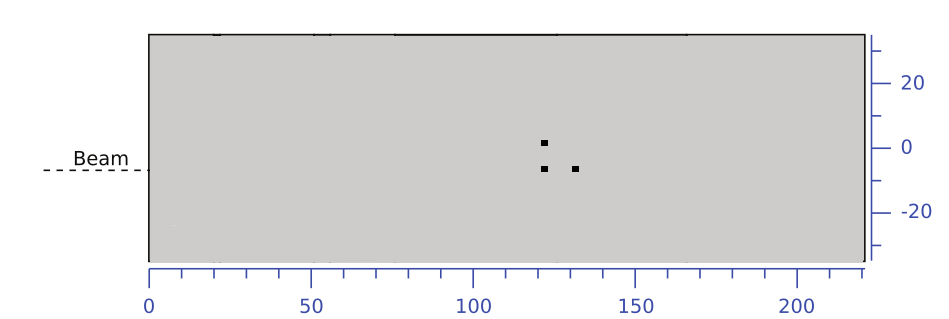
\includegraphics[scale = 0.3]{homo/homofant.png}
    \caption{Fantôme homogène}
    \label{fant homo}
\end{figure}{}



\openany
\subsubsection{Fantôme hétérogène}

Le fantôme est cette fois ci hétérogènes et représente un cas défavorable notamment à cause de l'interface entre les volumes (4) et (3) de la figure 3. Les trois volumes, toujours de la même taille, sont cette fois situé à 134~mm de profondeur pour ceux avant le pic de Bragg et à 144~mm pour celui dans le pic de Bragg. Le volume qui n'est pas dans l'axe du faisceau est excentré de 13~mm en dessous de l'axe. 

\begin{figure}[h]
    \centering
    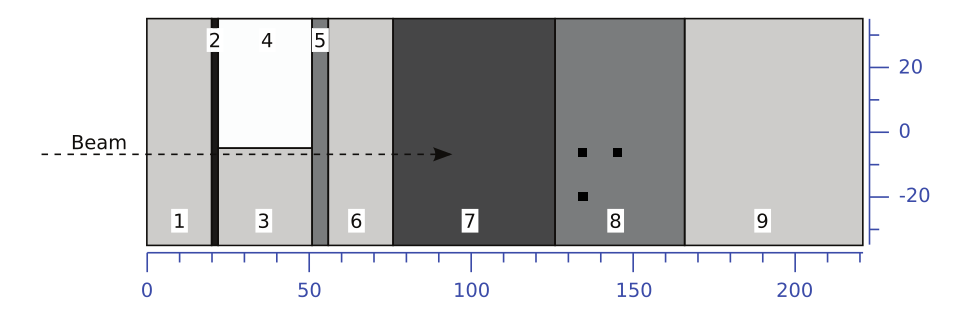
\includegraphics[scale = 0.3]{Parodi/heterofant.png}
    \caption{Fantôme composée en (1) (3) (6) et (9) de Polyethylène, en (2) d'os, en (4) de poumon, en (5) et (8) de muscle et en (7) de PMMA}
    \label{hetero phant}
\end{figure}{}

\subsubsection{Fantôme réaliste}

Le fantôme issu d'une image CT tête et cou est découpé en voxel de 2$^3$~mm on peut choisir de la même façon que précédemment les régions d’intérêts.

\subsection{Implémentation de l'information temporelle dans le vpgTLE}


\section{Résultats}

\subsection{\'Etude de la corrélation entre énergie et temps d'émission des gammas}

\subsubsection{Fantôme homogène}
\begin{figure}[h!]
\centering
\subfloat(a){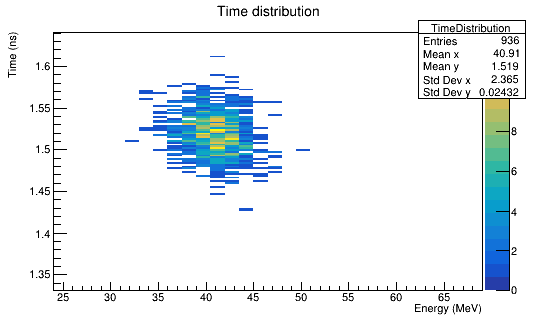
\includegraphics[scale=0.3]{homo/away.png}}
\subfloat(b){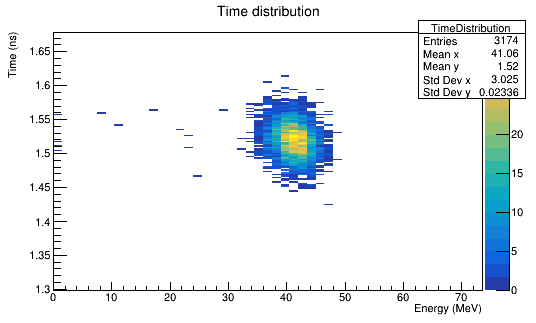
\includegraphics[scale=0.3]{homo/prebragg.png}}\\
\subfloat(c){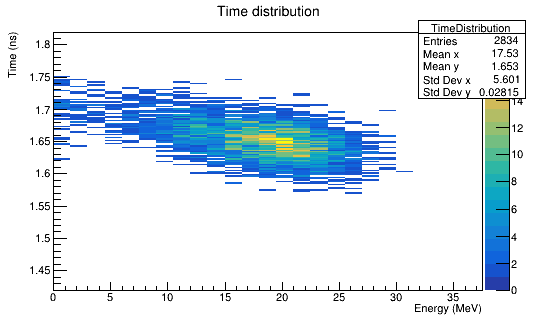
\includegraphics[scale=0.3]{homo/Bragg.png}}
\label{homo prot}
\caption{ Distribution des protons dans (a) un VoI éloigné du faisceau, (b) VoI dans le faisceau avant pic de Bragg et (c) VoI dans le pic de Bragg }

\end{figure}

\begin{figure}[h!]
\centering
\subfloat(a){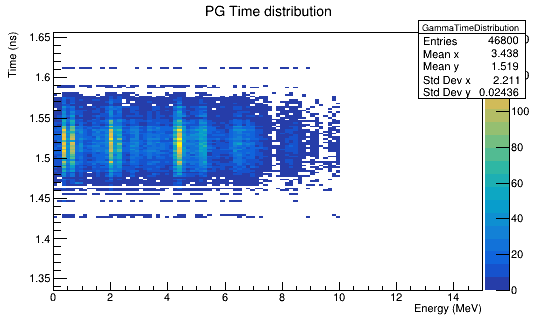
\includegraphics[scale=0.3]{homo/PG/away.png}}
\subfloat(b){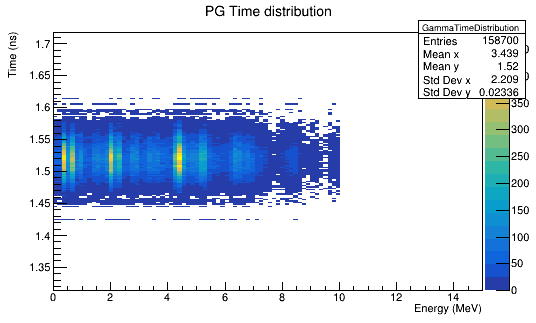
\includegraphics[scale=0.3]{homo/PG/preBragg.png}}\\
\subfloat(c){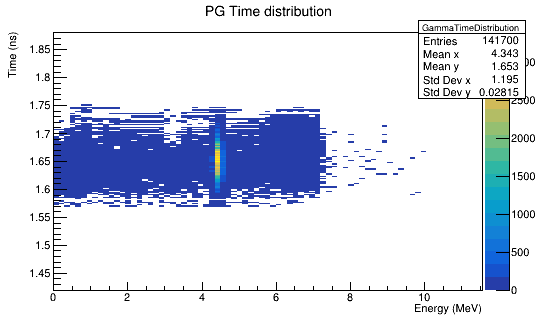
\includegraphics[scale=0.3]{homo/PG/postBragg.png}}
\label{homo pg}
\caption{ Distribution des gamma prompt dans (a) un VoI éloigné du faisceau, (b) VoI dans le faisceau avant pic de Bragg et (c) VoI dans le pic de Bragg }

\end{figure}{}


\subsubsection{Fantôme hétérogène}
\begin{figure}[h!]

\centering
\subfloat(a){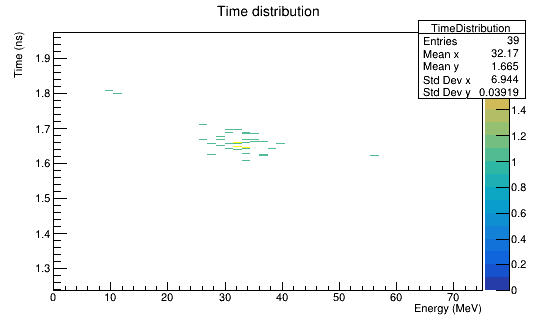
\includegraphics[scale=0.3]{Parodi/away.png}}
\subfloat(b){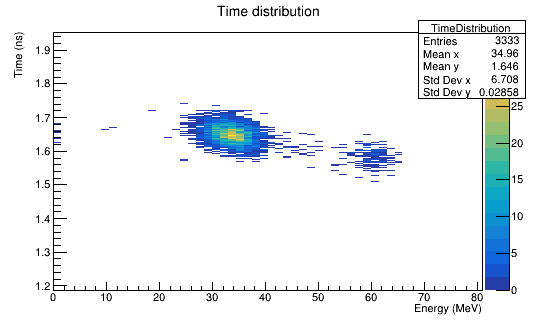
\includegraphics[scale=0.3]{Parodi/preBragg.png}}\\
\subfloat(c){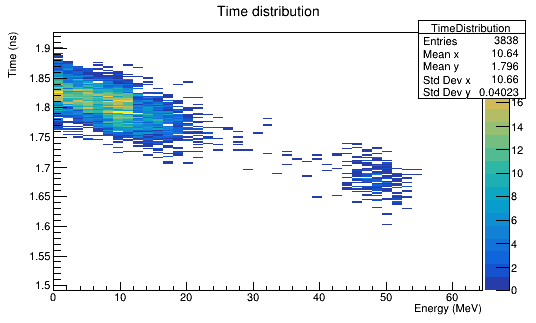
\includegraphics[scale=0.3]{Parodi/Bragg.png}}
\caption{ Distribution de protons dans (a) un VoI éloigné du faisceau, (b) VoI dans le faisceau avant pic de Bragg et (c) VoI dans le pic de Bragg }
\label{hetero prot}
\end{figure}

\begin{figure}[h!]

\centering
\subfloat(a){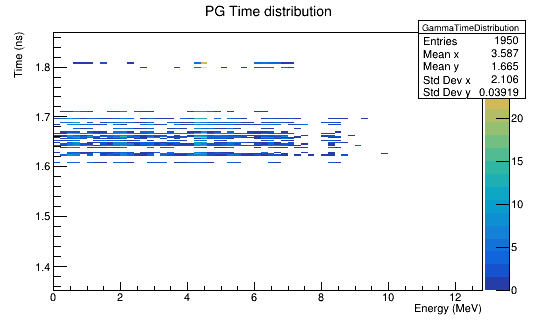
\includegraphics[scale=0.3]{Parodi/PG/away.png}}
\subfloat(b){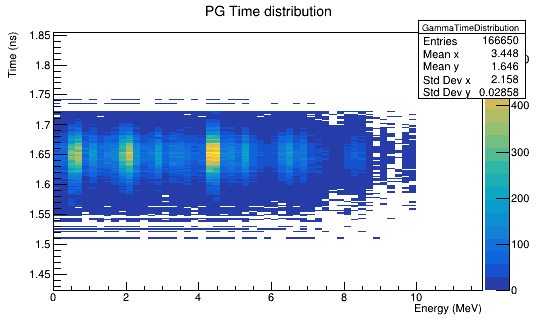
\includegraphics[scale=0.3]{Parodi/PG/preBragg.png}}\\
\subfloat(c){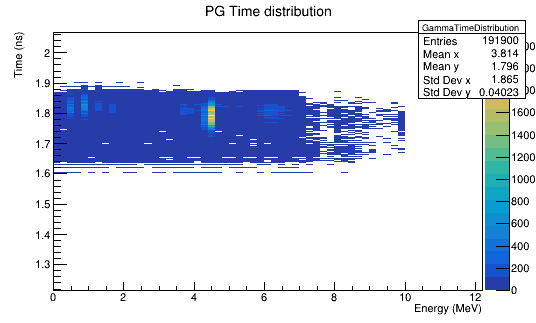
\includegraphics[scale=0.3]{Parodi/PG/Bragg.png}}
    
\caption{ Distribution de PG dans (a) un VoI éloigné du faisceau, (b) VoI dans le faisceau avant pic de Bragg et (c) VoI dans le pic de Bragg }
\label{hetero pg}
\end{figure}


\subsubsection{Fantôme réaliste}

\paragraph{Faisceau monoénergétique}

Fantôme issu d'un plan de traitement ORL représentant un cas réaliste présentant des hétérogénéités. Il est divisé en voxel de $2^{3}~mm^{3}$. 
  
\begin{figure}[h!]
\centering
\subfloat(a){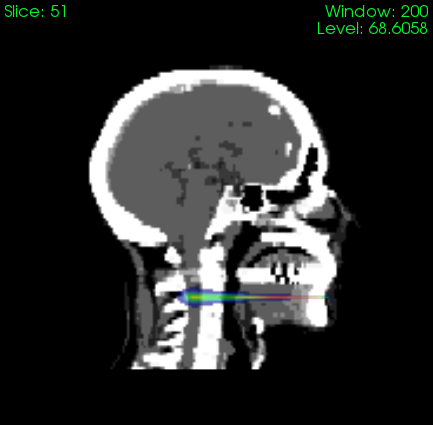
\includegraphics[scale=0.37]{CT/130/profil.png}}
\subfloat(b){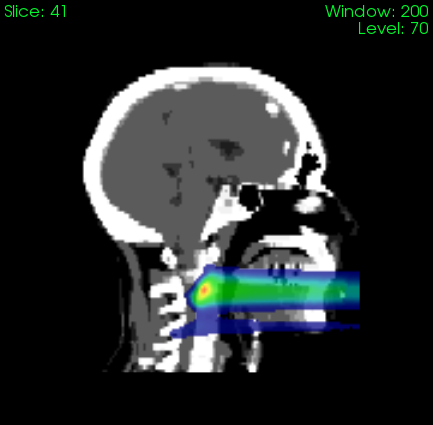
\includegraphics[scale=0.37]{CT/TPS/profil.png}}
\caption{Distribution de la dose dans le fantôme pour (a) le faisceau mono-énergétique de 130~MeV et (b) le faisceau issu du plan de traitement}
\label{profil}
\end{figure}



\paragraph{Faisceau issu d'un plan de traitement}
\begin{figure}[h!]
\centering
\subfloat(a){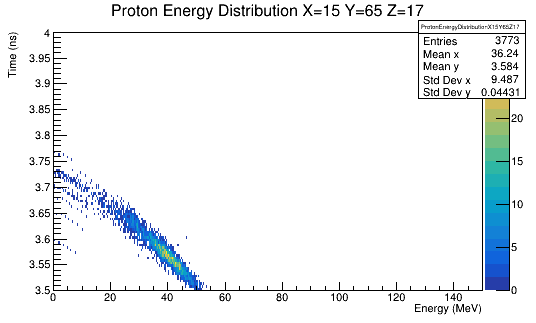
\includegraphics[scale=0.37]{CT/TPS/faisceauprot.png}}
\subfloat(b){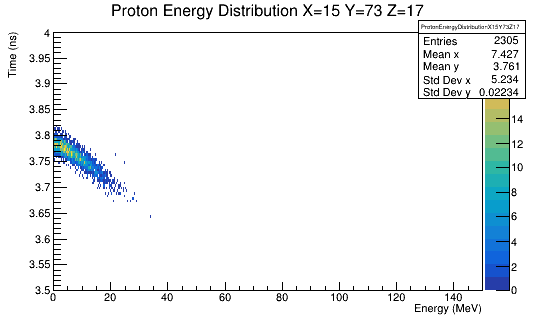
\includegraphics[scale=0.37]{CT/TPS/BraggProt.png}}
\caption{Distribution d'énergie de proton au milieu du faisceau (a) et au pic de Bragg (b)}
\label{tps prot}
\end{figure}

\begin{figure}[h!]
\centering
\subfloat(a){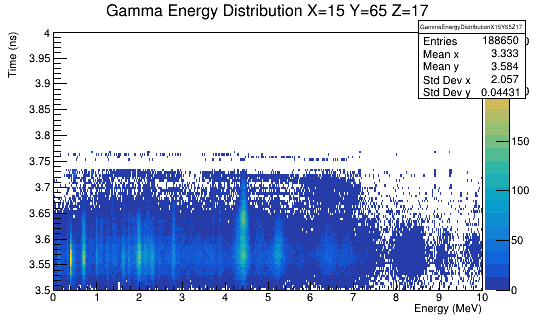
\includegraphics[scale=0.37]{CT/TPS/faisceaugamma.png}}
\subfloat(b){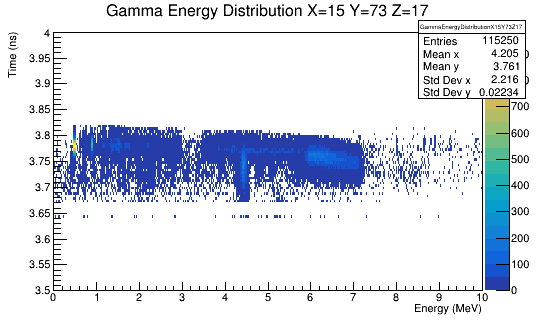
\includegraphics[scale=0.37]{CT/TPS/BraggGamma.png}}
\caption{Distribution d'énergie de gamma prompt au milieu du faisceau (a) et au pic de Bragg (b)}
\label{tps pg}
\end{figure}

\subsection{Implémentation de l'information temporelle dans le vpgTLE}

\section{Discussion}
\subsection{\'Etude de la corrélation entre énergie et temps d'émission des gammas}
Dans les trois cas de cette étude et pour tout les volumes nous trouvons un écart type de l'ordre de la dizaines de picosecondes. Or la résolution temporelle des détecteurs investigué dans le cadre de la collaboration CLaRys est de de 100~ps, dans cette limite nous stockerons donc le temps de vol indépendamment de l'énergie.  

\subsection{Implémentation de l'information temporelle dans le vpgTLE}


\bibliographystyle{apalike}
\bibliography{references}

\newpage

\appendix

\subsubsection{Résultats faisceau mono-énergétique A enlever ??}
\begin{figure}[h!]
\centering
\subfloat(a){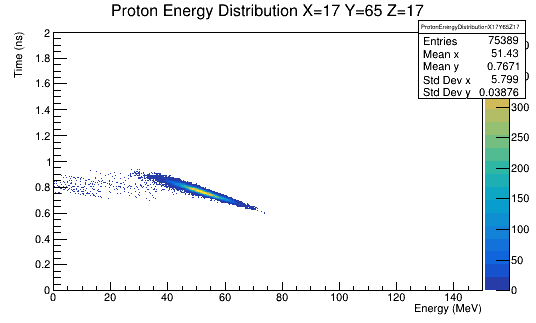
\includegraphics[scale=0.37]{CT/130/FaisceauProt.png}}
\subfloat(b){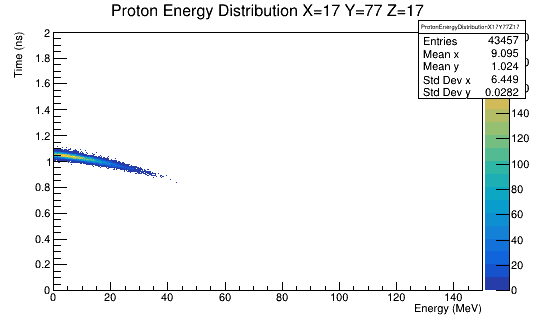
\includegraphics[scale=0.37]{CT/130/BraggProt.png}}
\caption{Distribution d'énergie de proton au milieu du faisceau (a) et au pic de Bragg (b)}
\label{130 prot}
\end{figure}

\begin{figure}[h!]
\centering
\subfloat(a){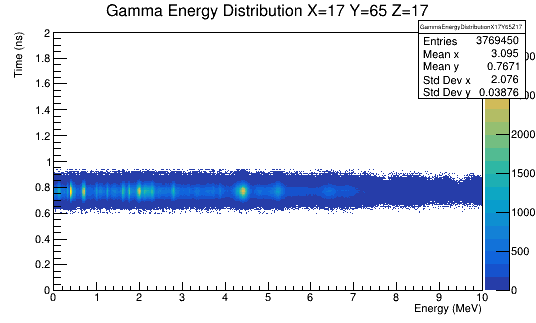
\includegraphics[scale=0.37]{CT/130/FaisceauGamma.png}}
\subfloat(b){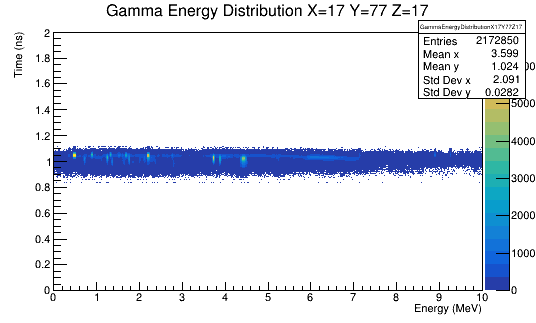
\includegraphics[scale=0.37]{CT/130/BraggGamma.png}}
\caption{Distribution d'énergie de gamma prompt au milieu du faisceau (a) et au pic de Bragg (b)}
\label{130 pg}
\end{figure}
\newpage

\end{document}
